% Instructions to change to html version:
% Comment out:
%  minipage, multicols,columnbreak, mathbf, hrule
% Replace all: \begin{minipage}% %%\end{minipage} %%%\begin{mulicols}  %%%\end{mulicols}  %%\columnbreak % %%\begin{framed} %%%\end{framed} %%%\hrule
% Search for \mathbf
% Replace \\] with \[ and \) with \(
% Enclose graphics in figure environments and add captions
% Re-tag \df environments as sections, subsections, etc.
% Command Line Code to Create html version:
%First: pdflatex -shell-escape filename.tex                                   
%Second, for each figure: inkscape "filename-figure1.pdf" -o "filename-figure1.png"
% Third: htlatex filename.tex "ht5mjlatex.cfg, charset=utf-8" " -cunihtf -utf8"


\documentclass[10pt]{article}

%\usepackage{tikz, pgf,pgfplots,wasysym,array}
%\usepackage{wasysym,array}

\usepackage{amsmath,amssymb}

\ifdefined\HCode
  \def\pgfsysdriver{pgfsys-tex4ht-updated.def}
\fi 
%\ifdefined\HCode
%  \def\pgfsysdriver{pgfsys-dvisvgm4ht.def}
%\fi 
\usepackage{tikz}
\usetikzlibrary{calc,decorations.markings,arrows}
\usepackage{pgfplots}

\pgfplotsset{compat=1.12}
\usepackage{myexternalize}
\usetikzlibrary{calc,decorations.markings,arrows}
\usepackage{framed}
\usepackage[none]{hyphenat}

\input{../../../common/1336_header_test.tex}

\begin{document}

\everymath{\displaystyle}



\newcommand{\ihat}{\boldsymbol{\hat{\textbf{\i}}}}
\newcommand{\jhat}{\boldsymbol{\hat{\textbf{\j}}}}
\newcommand{\khat}{\boldsymbol{\hat{\textbf{k}}}}

%\let\oldvec\vec
%\renewcommand{\vec}[1]{\oldvec{\mathbf{#1}}}

\renewcommand{\u}{\vec{u}}
\renewcommand{\v}{\vec{v}}
\newcommand{\w}{\vec{w}}
\renewcommand{\r}{\vec{r}}
\renewcommand{\a}{\vec{a}}
\renewcommand{\b}{\vec{b}}

\newcommand{\grad}{\vec{\nabla}}
\newcommand{\<}{\left\langle}
\renewcommand{\>}{\right\rangle}

\renewcommand{\myTitle}{MATH 2330: Multivariable Calculus}

\renewcommand{\mySubTitle}{Chapter 6 - Part 4: Line Integral Strategy}
%~\hfill Name: \underline{~~~~~~~~~~~~~~~~~~~~~~~~~~~~~~~~~~~~~~~~~~~~~~~}

\lectTitle{\vspace*{-.5in}\myTitle}{\vspace*{.1in}\mySubTitle \vspace*{-.25in}}


\section*{Types of Line Integrals:}% (Given a curve \(C\) with parametrization \(\vec{r}(t) = \<x(t), y(t)\>, \qquad a\leq t \leq b\))}

\setlength{\columnseprule}{0.4pt}
\setlength{\columnsep}{3em}

\hspace*{-.8in}%\begin{minipage}{1.25\textwidth}
%\begin{framed}

%Given a curve \(C\) with parametrization \(\vec{r}(t) = \<x(t), y(t)\>, \qquad a\leq t \leq b\)\\

\subsection*{Line Integral of a Scalar Function with respect to Arclength:}

\[
\int_C f(x,y)\ ds
\]

\textbf{Interpretation:} Net area under \(z=f(x,y)\) above the curve \(C\) in the \(xy-\)plane.\\

\textbf{Evaluate by:}
\begin{enumerate}[1.]
\item Sketch \& parametrize \(C\)
\item Replace \(x=x(t), \quad y=y(t), \quad ds = \sqrt{\left(\frac{dx}{dt}\right)^2+\left(\frac{dy}{dt}\right)^2}dt\)
\item Integrate wrt \(t\) from \(a\) to \(b\).

\end{enumerate}


\vspace*{.1in}%\hrule \vspace*{.2in}

\subsection*{Line Integrals with respect to  x and/or y:}


\[
 \int_C P(x,y)\ dx +  Q(x,y)\ dy
\]

\textbf{Evaluate by:}
\begin{enumerate}[1.]
\item Sketch \& parametrize \(C\)
\item Replace \(x=x(t), \quad y=y(t), \quad dx = x'(t)\ dt, \quad dy=y'(t)\ dt\)
\item Integrate wrt \(t\) from \(a\) to \(b\).


\end{enumerate}

\vspace*{.1in}%\hrule \vspace*{.2in}

\subsection*{Line Integrals over Vector Fields:}


\[
 \int_C \vec{F}\cdot d\vec{r}
\]

\textbf{Interpretation:} Work done by a force \(\vec{F}\) to move a particle along \(C\) from the starting point to the ending point.\\

\textbf{Evaluate by:}
\begin{enumerate}[1.]
\item Sketch \& parametrize \(C\)
\item Replace with \( \int_a^b \vec{F(t)}\cdot \vec{r}'(t)\ dt\)


\end{enumerate}

%\end{framed}

%\end{minipage}

\pagebreak

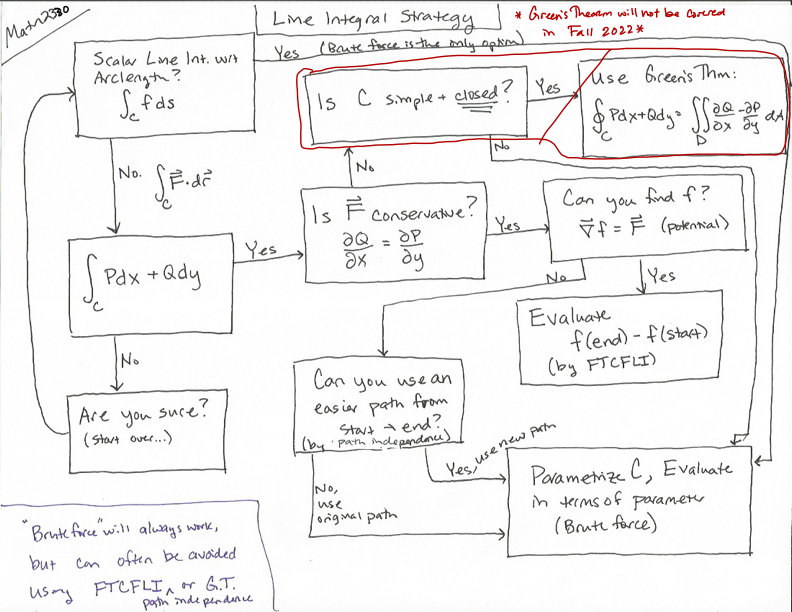
\includegraphics[angle=90,width=\textwidth]{22FQ-2330_Ch13_Flowchart.png}

\pagebreak

\section*{Miscellaneous Line Integral Problems}

\begin{enumerate}[{Problem }1.]

\item \(\int_C \frac{x\ dx + y\ dy}{\sqrt{x^2+y^2}}, \qquad C\): semi-circular arc of \(x^2+y^2 = 4\) from \((2,0)\) to \((-2,0)\).

\vfill

%\item \(\oint_C y^2\ dx + x^2\ dy, \qquad C\): square with vertices \((0,0)\), \((1,0)\), \((0,1)\), and \((1,1)\), counterclockwise %GT
%
%\vfill

\item \(\int_C x+2y\ ds, \qquad C\): parametrized by \(\vec{r}(t) = \<2-3t, 4t-1\>, \quad 0\leq t\leq 2\).

\vfill

\item \(\oint_C \left(x^2-y\right)\ dx + \left(y^2-x\right)\ dy, \qquad C\): circle of radius 5 centered at the origin, counterclockwise.

\vfill

\item \(\int_C 1+\frac{y}{3}\ ds, \qquad C\): parametrized by \(\vec{r}(t) = \<30\cos^3 t, 30\sin^3 t\>, \quad 0\leq t\leq \pi/2\).

\vfill

\end{enumerate}


\rotatebox{180}{
%\begin{minipage}{\textwidth}
\underline{Answers:}\\
\textbf{Problem 1:} 0, 
\textbf{Problem 2:} 50,
\textbf{Problem 3:} 0,
\textbf{Problem 4:} 225

%\textbf{Problem 2:} 0,
%\textbf{Problem 3:} 50,
%\textbf{Problem 4:} 0, 
%\textbf{Problem 5:} 225

%\end{minipage}
}


\end{document}

